% Muninn-X poster (Théo) — A0 portrait.  Build:  latexmk -pdf poster.tex
% Figures: python poster_theo/make_figures.py  (fig_*.pdf); paper Fig. 2 cropped into figures/muninn_fig2.png
\documentclass{article}
\usepackage[paperwidth=841mm,paperheight=1189mm,margin=20mm]{geometry}
\usepackage[fontsize=26pt]{scrextend}
\usepackage[T1]{fontenc}
\usepackage[utf8]{inputenc}
\usepackage[english]{babel}
\usepackage{newpxtext,newpxmath}
\renewcommand{\familydefault}{\rmdefault}
\usepackage{FiraSans}
\usepackage{amsmath,bm}
\usepackage[export]{adjustbox}
\usepackage{graphicx,xcolor,booktabs,array,enumitem}
\usepackage[most]{tcolorbox}
\usepackage[english,ruled,vlined,linesnumbered]{algorithm2e}

% ---------- colours (same palette as the figures) ----------
\definecolor{ink}{HTML}{0B0B0B}
\definecolor{muted}{HTML}{52514E}
\definecolor{navy}{HTML}{0D366B}
\definecolor{blue}{HTML}{2A78D6}
\definecolor{orange}{HTML}{EB6834}
\definecolor{aqua}{HTML}{1BAF7A}
\definecolor{paper}{HTML}{FCFCFB}
\color{ink}
\pagecolor{paper}

% ---------- boxes ----------
\newtcolorbox{pbox}[3][]{enhanced, colback=white, colframe=#2, boxrule=2.5mm, arc=6mm,
  left=12mm, right=12mm, top=8mm, bottom=8mm,
  fonttitle=\sffamily\bfseries\fontsize{44}{50}\selectfont, coltitle=white,
  colbacktitle=#2, toptitle=5mm, bottomtitle=5mm, lefttitle=12mm,
  before skip=0pt, after skip=0pt, title={#3}, #1}
\newtcolorbox{keybox}[1][blue]{enhanced, colback=#1!8, colframe=#1!8, boxrule=0pt, arc=4mm,
  left=8mm, right=8mm, top=5mm, bottom=5mm}

\newcommand{\hd}[1]{\par\smallskip{\sffamily\bfseries\large\color{navy}#1}\par\smallskip}
\setlist{nosep, leftmargin=1.1em, itemsep=6pt}
\setlength{\parindent}{0pt}
\setlength{\parskip}{6pt}
\SetAlFnt{\normalsize}
\SetAlCapFnt{\sffamily\bfseries}
\SetKwInput{KwIn}{Input}
\SetKwInput{KwOff}{Offline}

\newcommand{\E}{\mathbb{E}}
\newcommand{\Tc}{\mathcal{T}_{\text{cache}}}
\newcommand{\full}{^{\text{full}}}

\pagestyle{empty}
\begin{document}
% =====================================================================
% HEADER
% =====================================================================
\begin{tcolorbox}[enhanced, colback=navy, colframe=navy, arc=6mm, boxrule=0pt, before skip=0pt, after skip=0pt,
  left=16mm, right=16mm, top=10mm, bottom=10mm, height=112mm, valign=center]
\color{white}
\begin{minipage}[c]{0.77\linewidth}\raggedright
{\raggedright\sffamily\bfseries\fontsize{76}{86}\selectfont Muninn-X: certified caching for \emph{flow-matching} planners}\par\vspace{6mm}
{\sffamily\fontsize{36}{44}\selectfont What Muninn really guarantees, why the guarantee breaks, and how to fix it}
\end{minipage}\hfill
\begin{minipage}[c]{0.21\linewidth}\raggedleft
{\sffamily\fontsize{40}{48}\selectfont\bfseries Théo Palagi}\par\vspace{4mm}
{\sffamily\fontsize{28}{34}\selectfont MVA Master — Robotics\par 2026}
\end{minipage}
\end{tcolorbox}
\vspace{10mm}

% =====================================================================
% TOP HALF
% =====================================================================
\noindent
\begin{minipage}[t][530mm][t]{384mm}\vspace{0pt}
% ---------------------------------------------------------------- MUNINN
\begin{pbox}[height=530mm]{navy}{Muninn: reuse the network, with a guarantee}
\hd{The problem}
A diffusion planner (Diffuser, Decision Diffuser…) calls its denoiser $\varepsilon_\theta$ at each of its $T$ denoising steps: too slow for a control loop.
Muninn \emph{reuses} an already computed output at some steps, without retraining, and \textbf{certifies} that the plan $\tilde\tau_0$ stays close to the full-compute plan $\tau_0\full$:
\begin{keybox}[navy]
\[
\Pr\!\big[\, d(\tau_0\full,\tilde\tau_0) > \eta \,\big] \;\le\; \alpha
\]
\centering\small $\eta$: tolerance,\ \ $\alpha$: risk level,\ \ $d = \tfrac{1}{\sqrt H}\|\cdot\|_F$
\end{keybox}

\vspace{2mm}
\centering
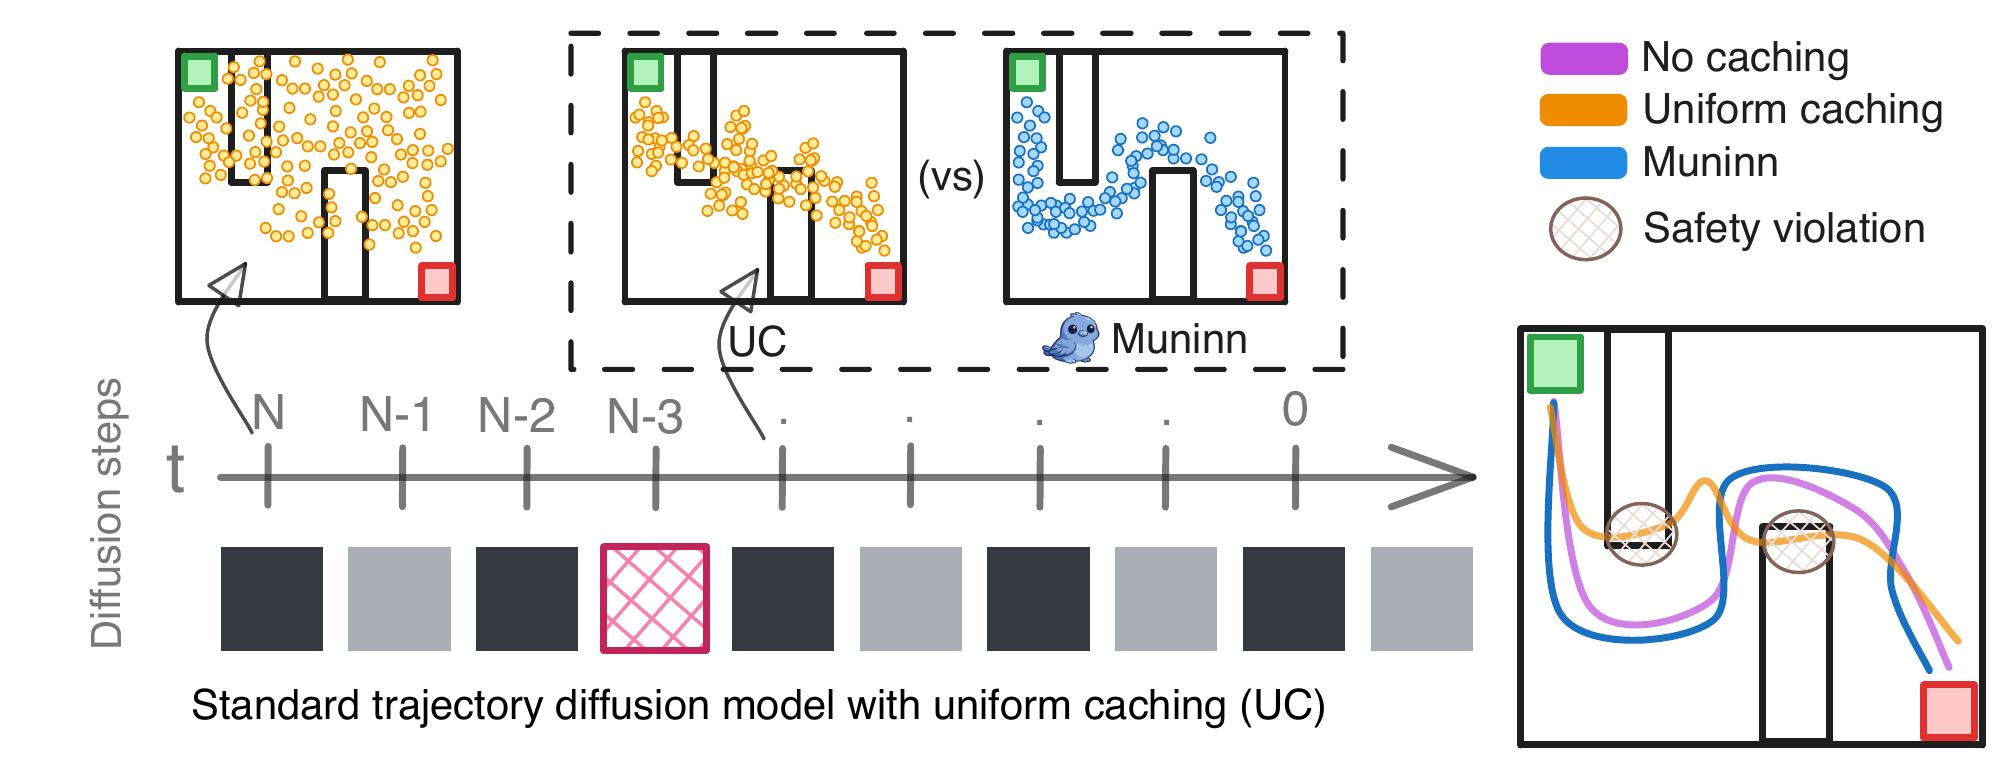
\includegraphics[width=\linewidth]{figures/muninn_fig2.png}\par\vspace{1mm}
\raggedright\small\color{muted}
\textbf{Fig.\ 2 of [1].} A mistaken reuse (red step) is not local: it is mixed into every later update and shifts the whole plan. Muninn decides \emph{per sample} where to reuse.
\normalsize\color{ink}

\hd{1.\ Sampler sensitivity}
Each step is Lipschitz (Assumption 1):
$\;\|\Delta_{t-1}\| \le K_t\|\Delta_t\| + L'_t\,\|e_t\|$,
with $\Delta_t$ the drift between the two chains and $e_t$ the network error, zero at recomputed steps. Unrolling:
\[
d \;\le\; \sum_{t\in\mathcal R} \underbrace{\Gamma L_t\|e_t\|}_{\text{cost } c_t},\qquad L_t = L'_t\prod_{j<t}K_j .
\]

\begin{minipage}[t]{0.49\linewidth}
\hd{2.\ Probe and calibration}
The network \emph{stem} gives features $F_t$ almost for free; a score $s_t$ measures how much $F_t$ changed.
On ``ghost'' chains, split conformal calibration gives a bound
$U(s) = \max\{m(s) + q_{1-\alpha/|\Tc|},\,0\} \ge \|e\|$.
\end{minipage}\hfill
\begin{minipage}[t]{0.47\linewidth}
\hd{3.\ Budget (Algorithm 1)}
$B \leftarrow \eta$. Reuse if $\hat c_t=\Gamma L_t U(s_t)\le B$, then $B\leftarrow B-\hat c_t$; otherwise recompute.
\begin{keybox}[navy]\small
\textbf{Reported:} up to $4.6\times$ faster (D4RL, AntMaze, Kitchen…) with \emph{no} risk violation.
\end{keybox}
\end{minipage}
\end{pbox}
\end{minipage}\hfill
\begin{minipage}[t][530mm][t]{405mm}\vspace{0pt}
% ---------------------------------------------------------------- BOX 1 : FM
\begin{pbox}[height=190mm]{blue}{1.\ Porting Muninn to \emph{flow matching}}
\hd{Flow matching (FM)}
Straight path from noise ($t=0$) to data ($t=1$): $x_t = t\,x_1 + (1-t)\,x_0$. The network learns the velocity $v_\theta(x,t)\approx \E[x_1-x_0\mid x_t=x]$, sampled with Euler:
\begin{keybox}[blue]
\[
x_{k+1} = x_k + h\,v_\theta(x_k,t_k)
\;\Rightarrow\; K_k = 1,\;\; L'_k = h .
\]
\end{keybox}
We cache $v$ instead of $\varepsilon$; the weights $L_k=h$ become \emph{constant}.

\hd{A first fix}
Read literally, the rule chains dozens of reuses: $p_{\text{viol}}\approx 1$. We score against the \textbf{last recompute} and calibrate lags $1\ldots10$.

\textbf{Testbeds:} 2D toys (MLP), then \textbf{Maze2D U-maze}: temporal U-Net, $128\times 6$ plans conditioned on start\,/\,goal.
\end{pbox}
\vspace{12mm}
% ---------------------------------------------------------------- BOX 2 : THE FLAW
\begin{pbox}[height=328mm]{orange}{2.\ Muninn's guarantee is wrong}
The last equality of Eq.\,(1) in [1] evaluates the network at the \emph{cached} state instead of the \emph{full} one, so the \textbf{drift} term disappears. The exact recursion is:
\begin{keybox}[orange]
\[
\Delta_{k+1} = (I + h\,\bar J_k)\,\Delta_k + h\,e_k
\;\Rightarrow\;
\Delta_N=\sum_k h\,M_{k+1\to N}\,e_k
\]
\end{keybox}
The paper sets $M = I$. In FM (Tweedie):
\[
\frac{\partial v}{\partial x}=\frac{1}{1-t}\Big[\frac{t}{(1-t)^2}\,\mathrm{Cov}(x_1\!\mid x_t)-I\Big]
\]
$\Rightarrow$ errors are \textbf{amplified on the boundaries between modes} (up to $900\times$). On the checkerboard, Muninn breaks its guarantee: $p_{\text{viol}}=0.083>\alpha=0.05$.

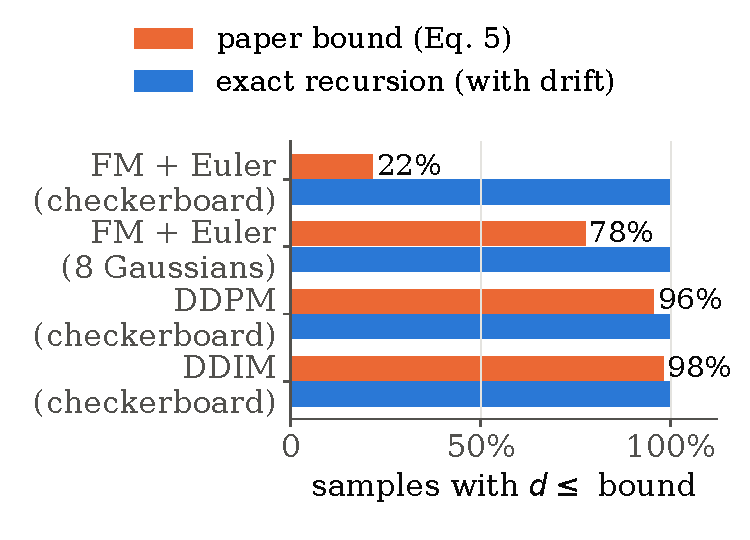
\includegraphics[width=0.45\linewidth,valign=t]{figures/fig_validity.pdf}\hfill
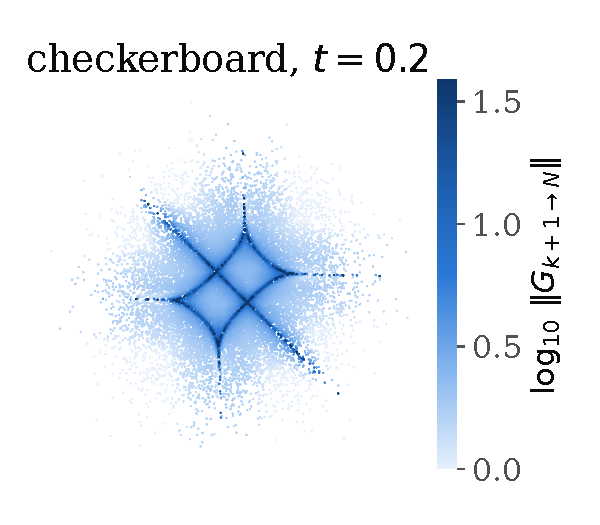
\includegraphics[width=0.37\linewidth,valign=t]{figures/fig_gmap.pdf}\par
\small\color{muted}
\textbf{Left:} oracle with exact errors, $\eta=0.05$ (DDPM/DDIM: $K_t=1/\sqrt{\alpha_t}$ over-counts propagation, which hides the gap). \textbf{Right:} amplification of an error made at $t=0.2$.
\end{pbox}
\end{minipage}

\vspace{12mm}
% =====================================================================
% BOTTOM HALF: OUR APPROACH
% =====================================================================
\begin{pbox}[height=485mm]{aqua}{Our approach: certify end to end, extrapolate where the flow forgets}
\begin{minipage}[t]{0.47\linewidth}
\hd{(a) Certify the final result, not each step}
Each method has \textbf{a single knob} $\theta$ (step count, budget, threshold). On $n=4000$ calibration chains, let $k_\theta$ = number of runs with $d>\eta$; keep the cheapest $\theta$ such that
\begin{keybox}[aqua]
\[
\Pr\!\big[\mathrm{Bin}(n,\alpha)\le k_\theta\big] \;\le\; \delta/|\Theta|
\]
\end{keybox}
(\emph{Learn-then-Test} + Bonferroni). Then, with probability $\ge 1-\delta$: $\Pr[d>\eta]\le\alpha$.
\textbf{No Lipschitz assumption}, for any caching policy. $d$ is measured against the exact ODE (RK4-400).

\hd{(b) Extrapolate instead of reusing}
Reusing $v$ with Euler is one big Euler step: \emph{always} worse than a uniform grid. We start from an AB2 base and extrapolate the velocity:
\[
v^{\text{ext}}_k = v_b + \tfrac{t_k-t_b}{t_b-t_a}\,(v_b - v_a).
\]

\hd{(c) A cost that sees the amplification}
\[
c_k = h\,\big\|G_{k+1\to N}\,e_k\big\|,\qquad G_{k+1\to N}=\textstyle\prod_{j>k}(I+hJ_j).
\]
A regressor $f_\phi$ predicts $\log c_k$ from \textbf{free signals} ($t$, lag, changes of $v$ and of $\hat x_1 = x+(1-t)v$). It is trained offline on random-decision chains, with $G\,e$ computed by Jacobian-vector products.
\end{minipage}\hfill
\begin{minipage}[t]{0.49\linewidth}
\vspace{4mm}
\begin{algorithm}[H]
\caption{Certified $G$-aware extrapolation}
\KwOff{train $f_\phi$; certify the threshold $\hat\tau$ with (a)}
\KwIn{$v_\theta$, context $c$, $N=100$, $\ell_{\max}=10$}
$x_0\sim\mathcal N(0,I)$; compute $u_0,u_1$; $\ell\leftarrow 0$\;
\For{$k = 2,\dots,N-1$}{
  $v^{\text{ext}}_k \leftarrow$ extrapolate from $(v_a, v_b)$\;
  $\varphi_k \leftarrow$ free signals\;
  \eIf{$f_\phi(\varphi_k)\le\hat\tau$ \textbf{and} $\ell<\ell_{\max}$}{
    $u_k \leftarrow v^{\text{ext}}_k$;\quad $\ell\leftarrow\ell+1$ \tcp*{0 NFE}
  }{
    $u_k \leftarrow v_\theta(x_k,t_k,c)$ \tcp*{1 NFE}
    $(v_a,v_b)\leftarrow(v_b,u_k)$;\quad $\ell\leftarrow 0$\;
  }
  $x_{k+1}\leftarrow x_k + h\big(\tfrac32 u_k - \tfrac12 u_{k-1}\big)$\;
}
\Return{$x_N$}
\end{algorithm}
\vspace{4mm}
\textbf{What we keep from Muninn:} per-step, per-sample decisions and a certified budget.
\textbf{What changes:} extrapolation instead of reuse, free signals instead of the probe, a $G$-aware cost instead of $L_t$, and certification on the final $d$.
\end{minipage}

\vspace{10mm}
{\color{aqua!60}\rule{\linewidth}{1.2mm}}
\vspace{2mm}

\begin{minipage}[t]{0.50\linewidth}\vspace{0pt}
\hd{Results on Maze2D U-maze (20\,000 test plans)}
\centering
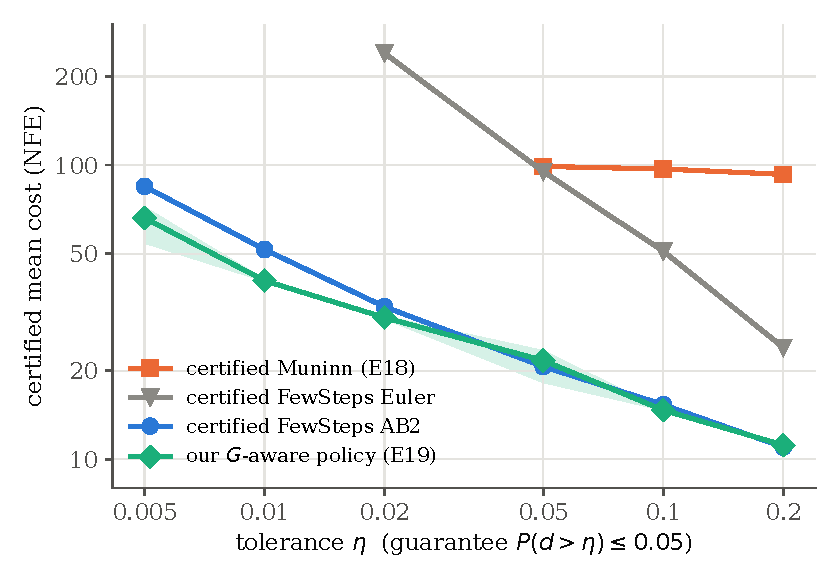
\includegraphics[width=0.68\linewidth]{figures/fig_maze.pdf}
\end{minipage}\hfill
\begin{minipage}[t]{0.47\linewidth}\vspace{4mm}
\begin{itemize}
\item \textbf{Certified Muninn} skips at most 7 of 100 steps and cannot certify $\eta\le 0.02$. AB2 is \textbf{$5$–$9\times$ cheaper}.
\item \textbf{Our policy} beats AB2 by $\mathbf{1.2}$–$\mathbf{1.3\times}$ at $\eta\le0.01$ (3 seeds), and ties beyond.
\item Without $G$ it \emph{loses} (97 vs 85 NFE at $\eta=0.005$); the probe adds nothing. Every method meets $\alpha$ on test.
\end{itemize}
\vspace{4mm}
\begin{keybox}[aqua]
\textbf{Take-away.} In FM, Muninn's guarantee must be redone end to end, and FewSteps AB2 is the real baseline. Per-sample adaptivity gives a real but modest gain, which comes from the amplification $G$, not from the probe.
\end{keybox}
\vspace{4mm}
{\footnotesize\color{muted}[1] \emph{Muninn: Your Trajectory Diffusion Model But Faster}, arXiv:2605.09999. \quad Code and notes: \texttt{Muninn-X}.}
\end{minipage}
\end{pbox}
\end{document}
